\chapter{Acondicionamiento ambiental}
\minitoc
\section{Condiciones de bienestar}
Las instalaciones de climatización deben proporcionar las condiciones óptimas de bienestar para que \emph{el mecanismo de regulación del cuerpo humano disipe el calor con el mínimo esfuerzo}.

La producción de calor por parte del ser humano crece en proporción a la intensidad de la actividad que desarrolla. La unidad de medida del calor metabólico es el \emph{Met} que equivale a 50 kcal/h m$^2$ y corresponde a una persona sentada inactiva.

\subsection{Condiciones atmosféricas que afectan el confort}

Los parámetros básicos que debe controlar un sistema de climatización son:
\begin{itemize}
	\item \emph{Temperatura del aire y superficiales}.
	En invierno se consideran temperaturas entre 18 y 23 °C, mientras que en verano se consideran desde 23 hasta 27 °C. A efectos prácticos, se considera 25 °C y 50\% en verano, y 22 °C y 50\% en invierno.
	\item \emph{Humedad relativa}. En general, la humedad relativa ideal para todo el año es de 50\%. No es conveniente que baje del 30\% dado que producen reacciones fisiológicas perjudiciales por una sensación de sequedad. Las humedades relativas superiores al 70\% no se deben tener debido a que son aún más perjudiciales.
	\item \emph{Movimiento del aire}. El movimiento del aire sobre el cuerpo humano incrementa la proporción de humedad y calor disipados, dando lugar a variaciones en las sensaciones de calor. Por ello, el movimiento del aire no debe ser excesivo, manteniendo valores entre 6 y 8 m/min en invierno, y de 8 a 12 m/min en verano.
\end{itemize}

\section{Sistemas de aire acondicionado}

Las instalaciones de aire acondicionado se puede clasificar según varios criterios \parencite{quadri2020}.
\begin{itemize}
	\item Según su misión:
	\begin{itemize}
		\item \emph{Para confort} humano
		\item \emph{Para procesos} industriales
	\end{itemize}
	\item Según la estación del año en que actúan:
	\begin{itemize}
		\item \emph{Instalaciones unificadas}, utilizadas para refrigeración y calefacción, actuando durante todo el año en forma coordinada.
		\item \emph{Instalaciones independientes}, utilizadas como solo refrigeración o solo calefacción, funcionando durante determinada temporada en el año.
		\item \emph{Instalaciones de AA de invierno previstas para verano}, con el fin de reducir la inversión inicial, son instalaciones para calefacción pero se dejan preparadas para instalar la planta de frío en un futuro.
	\end{itemize}
	\item Según el tipo de equipamiento:
	\begin{itemize}
		\item \emph{Expansión directa}, donde el refrigerante enfría directamente el aire en el espacio a acondicionar.
		\item \emph{Expansión indirecta o agua enfriada}, se utiliza agua como refrigerante secundario, la cual es enfriada previamente por un refrigerante primario. Luego, esta agua enfría el aire del ambiente que se desea acondicionar.
	\end{itemize}
	\item Según la forma de distribución de los fluidos:
	\begin{itemize}
		\item \emph{Unitarios}.
		\item \emph{Todo aire}.
		\item \emph{Todo refrigerante}.
		\item \emph{Todo agua}.
		\item \emph{Mixtos}
	\end{itemize}
\end{itemize}
\subsection{Normas de diseño}

Según indica el \citetitle[pág. 133]{quadri2007manual}, para seleccionar un aire acondicionado, se debe hacer un predimensionamiento con valores nominales y luego la verificación con las condiciones reales de operación.

De todas maneras, cada caso es particular y deben considerarse los datos ofrecidos por el fabricante.

\subsection{Sistemas unitarios}
Se trata de equipos autocontenidos de expansión directa instalados en el local a acondicionar \emph{sin la utilización de conductos}. Algunos se instalan en ventanas o paredes, mientras que otros son equipos portátiles que no requieren instalación.

\subsubsection{Equipo de ventana o pared}

Se denominan autocontenidos debido a que reúnen en forma completa en el interior todos los componentes necesarios para el tratamiento del aire. En este sistema no se implementan conductos para la distribución del aire. Está compuesto básicamente de los elementos que se indican \parencite{quadri2021sistemas}:
\begin{itemize}
	\item Gabinete o carcasa de montaje.
	\item Compresor hermético blindado, del tipo alternativo o rotativo para disminuir el ruido.
	\item Condensador y evaporador con serpentín de tubos de cobre y aletas de aluminio.
	\item Ventilador centrifugo para el evaporador y helicoidal para el condensador, con motor de accionamiento común.
	\item Sistema de calefacción por resistencia eléctrica o bomba de calor.
	\item Reja de inyección direccional de plástico.
	\item Reja de retorno desmontable para acceder a un filtro de aire.
	\item Termostato para regular la temperatura seleccionada por el usuario.
	\item Tubo capilar para la reducción de presión.
	\item Bandeja de eliminación de condensado.
\end{itemize}
La \autoref{fig:aire-ventana} muestra un esquema típico de este tipo de equipo. Se pueden ver dos zonas diferenciadas, la parte hacia el exterior y la que está hacia el interior del local. En la sección exterior se tiene el compresor, el condensador y el ventilador. En la sección interna se cuenta con el evaporador, el tubo capilar, las rejas de inyección y retorno, el filtro y el termostato.

\begin{figure}[h]
	\centering
	\caption{Esquema típico de un equipo individual de ventana o muro.}
	\label{fig:aire-ventana}
	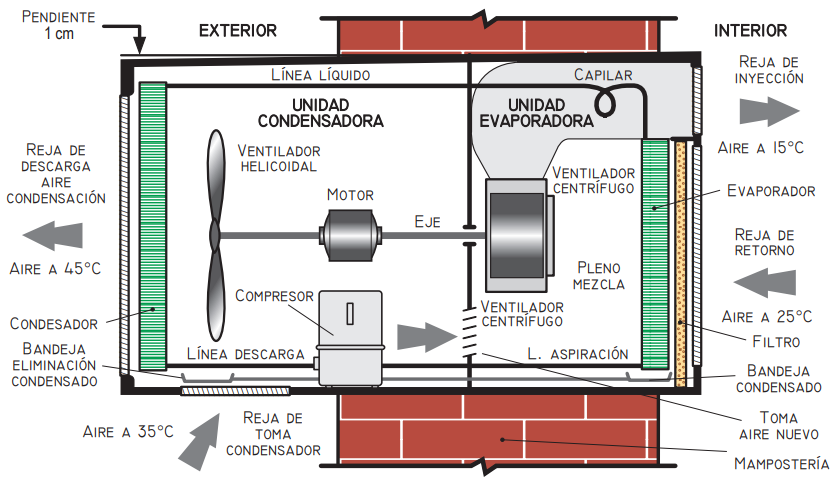
\includegraphics[width=0.8\linewidth]{acondicionamiento-ambiental/aire-ventana}
\end{figure}

En Argentina, los lugares más convenientes para instalar el equipo son al sur, sudeste o este, por la menor incidencia solar que hace mejorar el rendimiento de la unidad condensadora al trabajar a menor temperatura; no debiéndose colocar en lo posible sobre pared oeste y debe poseer adecuada circulación de aire en el condensador, evitando recirculaciones.

\emph{Este equipo se selecciona solamente en función de la carga térmica.}

\subsection{Sistema todo aire}

En este sistema el aire se trata en un recinto fuera del local y, posteriormente, \emph{se lo distribuye a los locales mediante conductos}, inyectándose mediante rejas o difusores. De esta manera, en los ambientes a acondicionar no hay equipos instalados.

Se diferencian de los sistemas unitarios porque el tratamiento de aire se realiza fuera del local y luego se distribuye mediante conductos.

\subsubsection{Equipos Roof-top}

Consisten en unidades similares a las de ventana, pero de mayor tamaño —aproximadamente, a partir de 7500 frigorías— y se instalan con conductos de distribución. Son diseñadas especialmente para instalaciones en intemperie y son adecuadas para locales de una sola planta con cubierta plana, tales como residencias, oficinas, supermercados, industrias, etc.

La selección se realiza considerando la carga térmica, la temperatura de entrada al condensador —adoptada como la temperatura exterior de bulbo seco— y la temperatura de entrada al evaporador —determinada por la mezcla del aire acondicionado con un cierto porcentaje de aire exterior—. Luego, se evalúa el caudal que debe desplazar el ventilador, verificando que la capacidad de extracción de calor sensible y latente no presente déficits significativos.

Por otra parte, al consultar catálogos de algunos fabricantes, se obtiene información sobre la capacidad de refrigeración y calefacción, el rendimiento, la presión estática externa (ESP) y el caudal del ventilador.

\subsubsection{Unidades de Tratamiento de Aire (UTAs)}

La UTA es la encargada de acondicionar el aire (filtrarlo, calentarlo, enfriarlo, humedecerlo o deshumidificarlo) antes de distribuirlo a los locales. Es un sistema modularizado y su configuración depende de los requerimientos particulares de cada proyecto. Los componentes más habituales son los siguientes:
\begin{itemize}
	\item Entrada de aire.
	\item Módulo de entrada, compuesta por filtros, ventilador y batería de precalentamiento.
	\item Módulo de mezcla.
	\item Módulo de acondicionamiento del aire, compuesto por baterías y/o resistencias eléctricas, deshumidificador, humectador y filtro anti gotas.
	\item Salida de aire.
\end{itemize}

\subsection{Sistema todo refrigerante}

También conocidos como equipos \emph{split} o sistemas separados, están compuestos por dos unidades: una interior, ubicada en el ambiente a acondicionar, y una exterior, responsable de disipar el calor hacia el exterior. Cuando el sistema cuenta con una sola unidad interior, se denomina \emph{simple split}; en cambio, si posee varias unidades interiores conectadas a una misma unidad exterior, se lo denomina \emph{multi split}. El aire es tratado mediante un sistema de expansión directa y circulado por ventiladores en el interior.

\subsection{Sistema todo agua}

En este sistema, el tratamiento del aire es de expansión indirecta con agua como refrigerante secundario. En los locales a acondicionar se colocan unidades terminales denominadas \emph{fan-coil}, constituidas por un ventilador y un serpentín donde circula el agua enfriada o calentada, la cual es transportada desde una \emph{unidad central} mediante cañerías y una bomba.

\subsubsection{Fan-coils}

Este sistema est\'a basado en instalar unos aparatos llamados fan-coils (serpent\'in y ventilador) en las habitaciones o locales que deben refrigerarse.

A los \textit{fan-coils} se hace llegar agua fr\'ia mediante una red de tuber\'ias proveniente de una central enfriadora. El agua llega al \textit{fan-coils} alimenta una bater\'ia cuya misi\'on es enfriar aire del local aspirado mediante un ventilador. En invierno la bater\'ia puede ser alimentada con agua caliente procedente de una caldera. La bater\'ia cuenta con purgadores y tapones en caso de querer realizar mantenimiento o inspecci\'on. Adem\'as, la unidad fan-coils cuenta con una bandeja de chapa galvanizada para el condensado.

Los sistemas de fan-coils se clasifican en base a dos criterios diferentes:
\begin{itemize}
	\item Que tenga o no toma de aire de ventilaci\'on. En este caso el sistema puede diseñarse de forma que el ventilador del fan-coils aspire aire \'unicamente del recinto o est\'a provisto de una toma de aire exterior.
	\item Seg\'un la disposici\'on y n\'umero de tubos de agua que acceden y salen del fan-coils. Esta disposici\'on puede ser de: dos tubos, tres tubos y cuatro tubos.
\end{itemize}

\subsubsection{Paneles radiantes}

Se trata de un sistema que impulsa agua caliente (entre los 40 y 45 \textcelsius) a trav\'es de un circuito de tuber\'ias que se colocan empotradas en el suelo. El calor emitido por las tuber\'ias se absorbe en el piso y posteriormente es emitido al recinto en forma de energ\'ia radiante y, en menor medida, convectiva.
\subsection{Sistemas mixtos}

En la práctica, los sistemas descritos anteriormente suelen combinarse con el sistema todo aire, en la medida que se instalen conductos de distribución en los locales \parencite[pág. 103]{quadri2020}. Así suelen combinarse, generalmente, los siguientes sistemas:
\begin{itemize}
	\item Agua-aire
	\item Refrigerante-aire
\end{itemize}
En estos sistemas, en los locales se emplean equipos similares a los fan-coil, alimentados con agua o refrigerante, complementados con la distribución de aire por conductos.

\subsubsection{Sistemas refrigerante-aire}

Se trata de sistemas de \textit{volumen de refrigerante variable}, conocidos por sus siglas \textit{VRV}. Se trata de un sistema de expansi\'on directa, basado en equipos de tipo multi-split, colocados en el espacio acondionado o pr\'oximos a \'el con todos los elementos necesarios para producir el enfriamiento del aire.

Su funcionamiento, en refrigeraci\'on, es el siguiente: en unidad exterior el fluido frigor\'ifico condensa y en estado l\'iquido y a alta presi\'on de condensaci\'on se reparte a las unidades interiores en donde se evapora enfriando el local. La transferencia de calor se realiza a trav\'es de los circuitos frigor\'ificos mediante tuber\'ias de refrigerante (una de l\'iquido y otra de gas) por cada pareja de m\'odulo exterior-interior. Aunque se puede dar el caso de que el sistema cuente con recuperaci\'on de calor, es decir que se utilice el calor sobrante de las unidades interiores para calefacci\'on de otras zonas que lo requieran. En este caso, la instalaci\'on contar\'a con tres tuber\'ias.

Las unidades interiores se presentan en una amplia gama de modelos diseñados para resolver las necesidades de cada ambiente, desde:
\begin{itemize}
	\item unidades terminales de montaje en pared (similares a los equipos split)
	\item tipo casette (para embutir dentro de los cielorrasos)
	\item tipo baja silueta (para embutir dentro de los cielorrasos y permitir distribuci\'on de aire mediante conductos)
\end{itemize}

\subsubsection{Chiller}
El chiller es un sistema enfriador de agua, la cual puede utilizarse en distintos procesos. En este caso particular, el agua enfriada se emplea en unidades fan-coil para climatizar ambientes.

El sistema consta de dos circuitos principales: uno de refrigerante y otro de agua. El refrigerante enfría el agua en el chiller, y esta agua es impulsada hacia los fan-coils, donde se absorbe el calor del aire del ambiente.

En algunos sistemas, la condensación del refrigerante se realiza mediante una torre de enfriamiento, lo que implica una condensación por agua. En ese caso, el sistema incorpora dos circuitos de agua (uno para enfriar el aire y otro para condensar el refrigerante) y un circuito de refrigerante.

\section{Selecci\'on de UTA}
Para seleccionar correctamente la UTA debemos conocer el caudal de aire de suministro ($\dot{V}$), la temperatura de entrada ($t_3$) y salida del aire de la UTA ($t_5$), la potencia frigor\'ifica ($N_R$) y la temperatura de roc\'io de la m\'aquina ($t_4$). Para esto hay que definir los par\'ametros conocidos y los que hay que hallar:
\begin{table}[H]
	\centering
	\caption{Par\'ametros para la selecci\'on de una UTA}
	\label{tab:parametros-seleccion-UTA}
	% \renewcommand{\arraystretch}{1.5}
	\begin{tabular}{p{0.8cm} l|p{0.5cm} l}
		\hline
		&\textbf{Par\'ametros conocidos} && \textbf{Par\'ametros a determinar} \\
		\hline
		$t_1$ & temperatura exterior & $\dot{V}$ & caudal de aire de suministro \\
		$\varphi_1$ & humedad relativa exterior & $t_4$ & temperatura de roc\'io de la UTA\\
		$t_2$ & temperatura interior & $t_5$ & temperatura del aire de suministro\\
		$\varphi_2$ & humedad relativa interior & $t_3$ & temperatura del aire a la entrada de la UTA\\
		$\dot{V}_V$ & caudal de ventilaci\'on & $N_R$ & potencia frigor\'ifica de la UTA\\
		$\dot{Q}_{se}$ & carga sensible del local & &\\
		$\dot{Q}_{le}$ & carga latente del local & &\\
		$f$ & factor de by-pass de la bater\'ia & &\\
		\hline
	\end{tabular}
\end{table}
Como los valores exteriores e interiores son conocidos situamos los puntos 1 y 2 en el diagrama psicrom\'etrico y trazamos la recta 1-2.
\subsection{Obtenci\'on de la temperatura de roc\'io ($t_4$)}
Para obtener $t_4$ se debe hallar el factor de calor sensible (FCS). Una vez realizado el balance t\'ermico de nuestro local, hallando el calor sensible total y el calor latente total podemos hallar el FCS con la \autoref{eq:factor-calor-sensible}.


\emph{Concepto extra.}\ Punto de referencia o foco: Est\'a situado a los 26,7 \textcelsius\ y 50\%\ de humedad relativa y se emplea junto con la escala de factores de calor sensible para dibujar las l\'ineas. 

Una vez obtenido el FCS, ubicamos en el diagrama psicrom\'etrico este valor y el punto de referencia y trazamos la recta. Luego, se traza una paralela a esta recta, que pase por el punto de condiciones interiores del local y se la prolonga hasta chocar la curva de saturaci\'on. Trazando una vertical descendente al punto obtenido por la intersecci\'on de las curvas se obtiene $t_4$.

\begin{figure}[H]
	\centering
	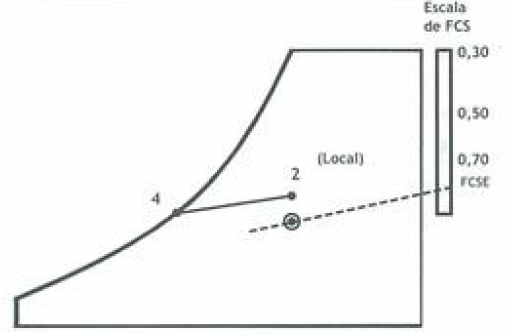
\includegraphics[width=0.5\linewidth]{acondicionamiento-ambiental/obtencion-temperatura-rocio.png}
	\caption{Obtenci\'on de temperatura de roc\'io}
	\label{fig:obtencion-temperatura-rocio}
\end{figure}

\subsection{Obtenci\'on del caudal de aire ($\dot{V}$)}

Con la siguiente ecuaci\'on se obtiene el volumen de aire de suministro para el local:

\begin{equation*}
	\dot{V}\ [\frac{m^3}{h}]= \frac{\dot{Q}_{se}[W]}{0,34\ (1-f)(t_2-t_4)}
\end{equation*}

\subsection{Obtenci\'on de la temperatura del aire a la entrada de la UTA ($t_3$)}
De la \autoref{eq:temperatura-mezcla} se obtiene la temperatura de la mezcla del aire de ventilaci\'on y el aire proveniente del local antes de entrar a la UTA. En este caso, $V_1$ pasa a ser $\dot{V}_V$ y $V_3$ pasa a ser $\dot{V}$, por lo tanto nos queda:
\begin{equation*}
	t_3=\frac{\dot{V}_V}{\dot{V}}\ (t_1-t_2)\ +\ t_2
\end{equation*}
El valor $t_3$ es la temperatura que tendr\'a la mezcla de aire exterior e interior, por tanto, el punto 3 se encuentra en la recta 1-2. 
\subsection{Obtenci\'on de la temperatura del aire a la salida de la UTA ($t_5$)}
Esto se realiza con la \autoref{eq:temperatura-suministro} obtenida de la definici\'on de by-pass.

Esta temperatura se encontrar\'a en la recta 2-4, es decir, que va de las condiciones interiores hasta las condiciones de saturaci\'on.
\subsection{Obtenci\'on de la potencia frigor\'ifica de la UTA}
Una vez ubicados los puntos 3 y 5 en el diagrama psicrom\'etrico se pueden hallar las entalp\'ias. Y mediante la siguiente formula se obtiene la potencia frigor\'ifica de la UTA:
\begin{equation*}
	N_R=0,33\ \dot{V}[m^3/h]\ (h_3 - h_5)[kJ/kg_a]
\end{equation*}
Una vez hallado todos los par\'ametros se hace uso de cat\'alogos de fabricantes y se selecciona la UTA.

\section{Distribución del aire}

\subsection{Tipos de distribución}
Las formas típicas de distribuir los caudales de aire acondicionado están relacionadas con la manera de regular el calor necesario a extraer en el funcionamiento de la instalación \parencite{quadri2020}. Analizando la \autoref{eq:caudal-de-circulacion}, como la temperatura del aire interior debe permanecer constante, se tienen dos posibilidades de variables a modificar si se requiere regular la cantidad de calor a extraer:
\begin{itemize}
	\item Temperatura de impulsión ($t_I$)
	\item Caudal circulante ($C$)
\end{itemize}

A partir de este hecho. el aire se puede distribuir a \emph{volumen constante}, manteniendo constante el caudal de aire circulante y variando la temperatura de impulsión, o a \emph{volumen variable}, variando el caudal de aire circulante y manteniendo constante la temperatura de impulsión.

Además de esta clasificación según el caudal y la temperatura del aire, los sistemas de distribución también pueden diferenciarse según la forma en que el aire se introduce y se mezcla en el ambiente. En este sentido, los sistemas pueden clasificarse en \emph{distribución por mezclado} y \emph{distribución por desplazamiento}.

\subsection{Distribución a volumen constante}

\subsubsection{Simple zona}
En los sistemas de volumen constante para una simple zona, se controla la temperatura del aire impulsado con el objetivo de alcanzar la temperatura de consigna en una única zona térmica, la cual puede estar compuesta por uno o varios locales con condiciones térmicas similares. Es una solución sencilla y eficiente para espacios con una carga térmica homogénea.

\subsubsection{Multi-zona}
En los sistemas multi-zona, la temperatura del aire ya no es única para todo el sistema, sino que se controlan de forma diferenciada varias zonas o locales con distintas necesidades térmicas. Esto permite una mayor flexibilidad y confort, adaptando el suministro de aire a las condiciones específicas de cada área. Se pueden implementar distintas estrategias de control:
\begin{itemize}
	\item \emph{Control con bombas de calor}, se suministra aire a la menor temperatura medida, y los locales que necesiten temperaturas más elevadas realizan un calentamiento adicional mediante bombas de calor.
	\item \emph{Post-enfriamiento}, el aire se impulsa a la mayor temperatura requerida entre las zonas, y luego se realiza un enfriamiento local adicional en los espacios que lo necesiten. Esta estrategia suele resultar más eficiente en términos energéticos.
\end{itemize}


\subsection{Distribución a volumen variable}

En los sistemas de distribución a volumen variable (VAV, por sus siglas en inglés), el caudal de aire se ajusta en función de la carga térmica de cada zona, utilizando compuertas reguladoras motorizadas o ventiladores con variación de velocidad.

Uno de los problemas de este sistema es que, al reducirse el caudal de aire para adecuarse a una menor demanda térmica, también disminuye el caudal de aire exterior destinado a la ventilación. Para evitar una ventilación insuficiente, se establece un límite mínimo de apertura en las compuertas, generalmente del orden del 15\%, que asegura un caudal constante de aire exterior, aun en condiciones de carga parcial \parencite{quadri2020instalaciones}.

\subsection{Distribución del aire por mezclado}

Consiste en introducir el aire impulsado en el ambiente a alta velocidad, de modo que se mezcle rápidamente con el aire interior, logrando una temperatura y calidad de aire relativamente uniforme en todo el espacio. Es el sistema más común en oficinas, locales comerciales y viviendas. 

A medida que el aire inyectado (aire primario) se aleja de la reja de alimentación, se va produciendo el \emph{arrastre y mezclado por inducción} del aire del ambiente (aire secundario), modificando su temperatura y humedad.


Para lograr un mezclado adecuado del aire, es fundamental considerar la ubicación de las rejas de alimentación y retorno. Si bien la posición de la reja de retorno no influye de forma significativa, su correcta ubicación sigue siendo importante, debiendo considerarse que \emph{no se produzcan cortocircuitos} del aire entre ambas bocas.


En general, las rejas de alimentación se colocan en la parte superior del espacio. Lo que respecta a las rejas de retorno, la mejor disposición es en la pared opuesta a las rejas de alimentación y en la zona inferior\footnote{No pegadas al suelo porque arrastran polvo y suciedad}. Aunque debe aclararse que no importa si una boca de retorno está al lado de una de alimentación, en la medida que se inyecte el aire a una velocidad adecuada, como sucede en los equipos individuales.

\subsection{Distribución del aire por desplazamiento}
El aire se introduce a baja velocidad desde zonas cercanas al suelo. Al estar más frío, desplaza el aire caliente y contaminado hacia arriba, que luego es extraído por rejillas en la parte superior. Es más eficiente desde el punto de vista energético y de la calidad del aire, pero requiere un diseño más cuidadoso. La velocidad del aire de difusión es pequeña y necesita difusores especiales.

\section{Rejas y difusores}

\subsection{Rejas de alimentación}

Se ubican en la pared o conductos, inyectando el aire en forma horizontal. Deben ser capaces de tener tres tipos de regulación: direccional horizontal, vertical y de caudal.


Para la selección de las rejas de alimentación debe tenerse en cuenta el caudal de aire y el alcance que debe tener \parencite{quadri2020instalaciones}. El \emph{alcance} se define como la distancia horizontal recorrida desde la reja por el aire primario, hasta obtener un valor mínimo de movimiento y comenzar a caer sobre un plano de $1.80$ m de altura, ubicado desde $3/4$ hasta la pared opuesta.


\emph{Se busca que el aire secundario no alcance velocidades molestas para las personas.}


A efectos prácticos, el alcance se considera desde la reja hasta la pared opuesta. Si se tienen dos rejas enfrentadas, el alcance será la mitad de la distancia entre ambas.

La \autoref{tab:rejas} se utiliza para la selección de las rejas de alimentación en función del caudal y el alcance. Indica las dimensiones de la reja: ancho y alto.

\begin{table}[H]
	\centering
	\caption{Tabla de selección de rejas de inyección (cm).}\label{tab:rejas}
	\begin{tabular}{c|ccccccc}
		\hline
		Caudal & \multicolumn{7}{c}{Alcance del aire en metros} \\
		m$^3$/min & 3 & 4,2 & 5,4 & 6,6 & 7,8 & 9 & 10,2 \\ \hline
		2,1 & 20$\times$10 & & & & & & \\
		2,8 & 20$\times$10 & 20$\times$10 & & & & & \\
		4,2 & 30$\times$10 & 20$\times$10 & 20$\times$10 & 20$\times$10 & & & \\
		5,6& 35$\times$15 & 25$\times$10 & 25$\times$10 & 20$\times$10 & 20$\times$10 & 20$\times$10 & \\
		7 & & 35$\times$15 & 35$\times$10 & 30$\times$10 & 30$\times$10 & 25$\times$10 & 25$\times$10 \\
		8,4 & & 40$\times$15 & 30$\times$15 & 30$\times$15 & 30$\times$10 & 30$\times$10 & 30$\times$10\\
		9,8 & & 60$\times$15 & 40$\times$15 & 35$\times$15 & 30$\times$15 & 35$\times$10 & 35$\times$10 \\
		11,2 & & 60$\times$20 & 50$\times$15 & 40$\times$15 & 35$\times$15 & 35$\times$15 & 35$\times$15\\
		12,6 & & 60$\times$20 & 60$\times$15 & 50$\times$15 & 40$\times$15 & 40$\times$15 & 35$\times$15\\
		14 & & 60$\times$25 & 60$\times$20 & 60$\times$15 & 40$\times$15 & 40$\times$15 & 35$\times$15\\
		15,4 & & 75$\times$25 & 60$\times$20 & 60$\times$15 & 60$\times$15 & 40$\times$15 & 40$\times$15\\
		16,8 & & & 75$\times$20 & 60$\times$20 & 60$\times$15 & 40$\times$15 & 40$\times$15\\
		18,2 & & & 75$\times$25 & 75$\times$20 & 70$\times$15 & 50$\times$15 & 50$\times$15\\
		19,6 & & & 75$\times$25 & 75$\times$20 & 70$\times$15 & 60$\times$15 & 60$\times$15 \\
		\hline
	\end{tabular}
\end{table}

También, se puede usar la tabla del manual para la selección, en función del caudal y el alcance \parencite[pág. 205]{quadri2007manual}.

\subsection{Rejas de retorno}

Captan el aire del ambiente, por lo que no requieren regulación direccional y sólo es necesario que cuenten con regulación volumétrica.

Se dimensionan en función del caudal de aire ($C$) que debe absorber y la velocidad del aire ($V$). Este último se adopta de tal manera que no sea molesto ni ruidoso para las personas. Generalmente, se adopta una velocidad entre 90 y 120 m/min. 

El área de la reja de retorno se calcula como:
\begin{equation}
	A = \dfrac{C}{V}
\end{equation}


\subsection{Difusores}

Distribuyen el aire en varias direcciones, normalmente desde el techo. Logran una mezcla más uniforme del aire en el ambiente. Se usan mucho en oficinas y locales para un confort térmico más parejo.

Su selección es similar a la de rejas de inyección, pero en este caso el alcance es radial y se denomina como \emph{radio de difusión}. La \autoref{tab:difusores} permite la selección de los difusores en función del caudal y el radio de alcance.

\begin{table}[H]
	\centering
	\caption{Tabla de selección de difusores (diámetro en cm).}\label{tab:difusores}
	\begin{tabular}{c|cccccccccc}
		\hline
		Caudal & \multicolumn{7}{c}{Radio de alcance en metros} \\
		m$^3$/min & 0,5 & 1 & 2 & 2,5 & 3 & 3,5 & 4,5 & 5 & 5,5 & 6 \\
		\hline
		1    & 12 & 12 &    &     &     &     &     &     &    &    \\
		1,5  & 15 & 12 & 12 &     &     &     &     &     &    &    \\
		2    & 15 & 15 & 15 &     &     &     &     &     &    &    \\
		3    &    & 15 & 15 & 15  &     &     &     &     &    &    \\
		3,5  &    & 20 & 20  & 20  & 20  &     &     &    &     &    \\
		4    &    & 20 & 20  & 20  & 20  & 20  &     &    &     &    \\
		5    &    & 25 & 20  & 20  & 20  & 20  & 20  &    &     &    \\
		6    &    & 25 & 25  & 25  & 25  & 25  & 25  & 20 & 20  &    \\
		7    &    & 30 & 25  & 25  & 25  & 25  & 25  & 20 & 20  & 20 \\
		8    &    & 30 & 30  & 25  & 25  & 25  & 25  & 20 & 20  & 20 \\
		8,5  &    & 40 & 30  & 30  & 30  & 30  & 30  & 25 & 25  & 20 \\
		10   &    & 45 & 40  & 30  & 30  & 30  & 30  & 25 & 25  & 20 \\
		14   &    & 50 & 45  & 40  & 30  & 30  & 30  & 25 & 25  & 25 \\
		17   &    &    & 50  & 45  & 40  & 40  & 30  & 30 & 30  & 30 \\
		20   &    &    & 50  & 45  & 40  & 40  & 40  & 30 & 30  & 30 \\
		\hline
	\end{tabular}
\end{table}

También se pueden seleccionar a partir de los gráficos del manual \parencite[pág. 207 y 208]{quadri2007manual}, pero aparenta presentar errores.
\section{Conductos}

Los conductos más empleados están fabricados con chapa de hierro galvanizado. En su diseño deben tenerse en cuenta factores como transformaciones, codos, acoplamientos, obstáculos, entre otros.

\subsection{Modificación de la forma del conducto}
Cuando se reduce la sección de un conducto rectangular, la inclinación de las paredes no debe superar el 25\%, y la disminución de su área no debe exceder el 20\%.

En caso de ampliación, ya sea por requerimientos del sistema o para la instalación de elementos como baterías de calefacción, la inclinación del conducto debe ser, como máximo, de 30° antes del elemento y de 45° después de este.

Si existe un obstáculo en el interior del conducto, se debe colocar una cubierta que guíe el flujo de aire rodeando dicho obstáculo. Si esta cubierta ocupa más del 20\% de la sección del conducto, se debe realizar una bifurcación que mantenga el área total del flujo constante.

\subsection{Codos}

Los codos pueden ser de sección circular y rectangular. Para los codos rectangulares se establece que el radio interno de curvatura ($R_i$) debe ser mayor o igual a 3/4 partes del ancho del conducto ($D$):
\begin{equation}
	R_i \geq 3/4 D
\end{equation}
Para radios internos menores, se colocan guiadores. Su selección se detalla en la página 186 del manual \parencite{quadri2007manual}.

\subsection{Diseño de conductos}

Se calcula según el caudal de aire en circulación y el gradiente hidraulico R.

Existen dos métodos de trabajo para la selección de conductos: i) el método de fricción constante, y ii) sección o diámetro constante.

El método de \emph{fricción constante} se basa en la suposición de un gradiente hidráulico $R$ uniforme a lo largo de toda la canalización. La experiencia práctica ha demostrado que este método es sencillo y ofrece resultados satisfactorios.

Se utiliza la gráfica de la \autoref{fig:diseño-conductos}, y el procedimiento consiste en determinar el gradiente $R$ a partir del caudal máximo transportado, fijando una velocidad máxima de circulación. A partir de este punto se obtiene el diámetro del tramo principal, lo que da origen a la denominada recta de maniobra. Desde esta recta de $R$ constante se determinan los diámetros del resto de los conductos, en función de los caudales que circulan por cada uno de ellos, y las velocidades a las que lo harán.

\begin{figure}
	\centering
	\caption{Ábaco para el diseño de conductos de sección circular.}
	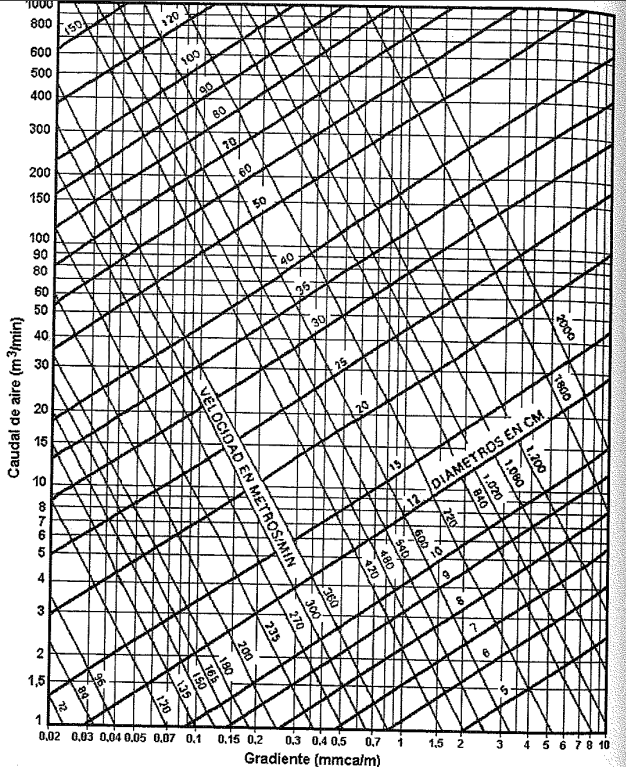
\includegraphics[width=0.5\linewidth]{acondicionamiento-ambiental/abaco-conducto}
	\label{fig:diseño-conductos}
\end{figure}

\subsubsection{Conductos de sección rectangular}
Cuando se requiere el uso de conductos rectangulares, se puede utilizar un ábaco de conversión que permite transformar un conducto circular en uno rectangular (\autoref{fig:conversion-conducto}). Como norma práctica, se recomienda que los conductos rectangulares se aproximen lo más posible a una forma cuadrada, evitando que la variación de lados exceda la relación de 5 a 1.

En el ábaco, dado el diámetro del conducto circular y uno de los lados del conducto rectangular, se puede determinar el otro lado correspondiente.

\begin{figure}
	\centering
	\caption{Ábaco para la conversión de conductos de sección circular a rectangular.}
	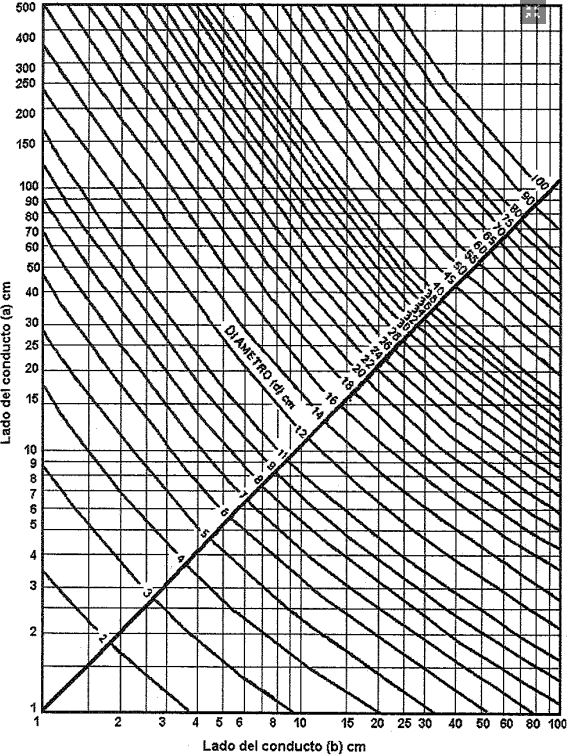
\includegraphics[width=0.5\linewidth]{acondicionamiento-ambiental/conversion-conducto}
	\label{fig:conversion-conducto}
\end{figure}
\subsubsection{Verificación de la caída de presión del ventilador}

Una vez definidos los ductos y sus componentes, es necesario verificar que la caída de presión total no supere la presión disponible proporcionada por el ventilador. Para ello, se utiliza la siguiente ecuación, que corresponde al cálculo de la pérdida de carga en función de la fricción y la longitud, como se realiza en mecánica de fluidos y máquinas fluidodinámicas:

\begin{equation}
	H_v = 2 \sum I \cdot R + \sum Z
\end{equation}

Donde:

\begin{itemize}
	\item $H_v$ es la presión total que debe vencer el ventilador para transportar el aire a la velocidad especificada hasta los puntos extremos del sistema.
	\item $2 \sum I \cdot R$ representa la pérdida de carga total debida a la fricción en los tramos rectos y en los accesorios, correspondiente al recorrido más desfavorable.
	\item $\sum Z$ incluye las pérdidas localizadas causadas por elementos como rejillas, persianas, filtros, baterías, entre otros.
\end{itemize}

El valor de presión disponible debe ser proporcionado por el fabricante del equipo.

\section{Ventiladores}

Los ventiladores son elementos de la instalación cuya función es aumentar la presión del aire dentro de los conductos. Se clasifican principalmente en \emph{axiales} y \emph{centrífugos}.

En los ventiladores centrífugos, el aire ingresa por una boca ubicada en el eje de rotación, sigue una trayectoria envolvente alrededor de dicho eje y sale impulsado en una dirección perpendicular (90°), debido a la fuerza centrífuga, de ahí su nombre. Estos ventiladores pueden clasificarse según la disposición de sus paletas en: curvadas hacia adelante, curvadas hacia atrás y radiales. Son equipos de alto rendimiento y adecuados para manejar presiones relativamente elevadas.

En los ventiladores axiales, el aire ingresa y sale en la misma dirección que el eje del ventilador. Se dividen en helicoidales y axiales propiamente dichos.

Los ventiladores \emph{helicoidales} tienen palas anchas, con gran superficie de empuje. Se utilizan comúnmente para extracción de aire o en aplicaciones donde las resistencias al flujo son muy bajas.

Por otro lado, los ventiladores \emph{axiales propiamente dichos} poseen palas más angostas, lo que les permite alcanzar mayores presiones, capacidades y consumos eléctricos similares. Existen también versiones reversibles, que pueden funcionar tanto como extractores como impulsores.